\documentclass{article}

\usepackage[cmex10]{amsmath}
\usepackage{amssymb}
\usepackage{amsthm,bm,array,psfrag,graphicx}
\usepackage[nolist]{acronym}
\usepackage{cite}
\usepackage{float}
\usepackage{caption}
\usepackage{subcaption}
\usepackage{booktabs}

\title{An Interface Between Digital and Analog: Bridging Software and Hardware}
\author{Raquel G. Machado and Alexander M. Wyglinski and Robin Getz}


\begin{document}
\maketitle

\section{Introduction}
Several software defined radio (SDR) \cite{mitola,sdr1,speakeasy} architectures have been developed and are commercially available in order to enhance the prototyping phase of new wireless technologies as well as advance the current state-of-the-art in wireless and networking communications systems. While there exists several well-known SDR platforms that are commercially available \cite{USRP,KUAR,Motorola,Maynooth,Rice}, many of these systems are designed primarily for conducting fundamental research and experimentation, and not for development into actual commercial products and prototypes. The creation of new SDR prototyping platforms and their accompanying software interfaces is the key for enabling continued advances in the wireless sector and to better understand both the capabilities and limitations of SDR technology when used in real-life communications systems. These are other factors to discuss: \cite{survey, hardware,path}

Within this context, the FMCOMMS1 high-speed analog module \cite{FMCOMMS} was designed to demonstrate the latest generation of high-speed data converters. The FMCOMMS1 module displays sampling-level processing capabilities of 1GS/s and enables radio frequency (RF) applications across a wide frequency range. In addition, it is customizable across software, and without any hardware changes it is possible to use different configurations that can be applied in many different communications applications. Although ADI's FMCOMMS1 module is currently available to the community, there does not presently exist any software support for these products in terms of a software environment for communications system design  and prototyping, e.g., GNU Radio \cite{GNU}, that can enable the community to use these platforms for over-the-air experimentation.

\section{Software Defined Radio Overview}

\subsection{Existing Software Defined Radio Platforms}

One of the most well-known SDR hardware platform is the Universal Software Radio Peripheral (USRP). The USRP is a device developed by Ettus Research LLC, which turns general purpose computers into flexible SDR platforms. The core of the USRP is a motherboard with four high-speed ADCs and DACs and a FPGA. The ADCs/DACs are connected to the radio Front-Ends (called daughterboards), while the FPGA is connected to a general purpose computer. In the Universal Software Radio Peripheral - Version 1 (USRP1) this connection is performed by an USB port, while the USRP2 includes a Gigabit ethernet interface. The main principle behind the USRP is that the digital radio tasks are divided between the internal FPGA and the external host CPU. The high speed general purpose processing, like down and up conversion, decimation, and interpolation are performed in the FPGA, while waveform-specific processing, such as modulation and demodulation, are performed at the host CPU. The USRP platform can be used with both GNU radio and MATLAB software development environments.

Another well-known SDR hardware platforms is the Kansas University Agile Radio (KUAR). The KUAR platform was designed to be a low-cost experimental platform
targeted at the frequency range 5.25 to 5.85 GHz and a tunable bandwidth of 30MHz. The platform contains a Xilinx Virtex-II Pro FPGA board and a PCI Express 1.4 GHz Pentium-M microprocessor. With these features, almost all process can be implemented in the platform, instead of the host computer, which minimizes the host-interface requirements. In addition, the KUAR utilizes a modified form of the GNU Radio software framework to complete the hardware platform.

With respect to compact SDR platforms, the Maynooth Adaptable Radio System (MARS) was designed to be connected to a personal computer where all the signal processing algorithms are to be implemented. Another objective was to deliver a
performance equivalent to base station and the wireless communication standards in the frequency 1700 to 2450 MHz. The software framework selected for initial development was the IRiS framework (Implementing Radio in Software).

Some other SDR platforms include:

\begin{itemize}
\item Berkeley BEE2: has five Xilinx Virtex-II Pro FPGAs on a custom-built emulation board.
\item Japanese National Institute of Information and Communications Technology (NICT) SDR Platform: contains two embedded processors, four Xilinx Virtex2 FPGA, and RF modules that could support 1.9 to 2.4 and 5.0 to 5.3 GHz.
\item Rice University Wireless Open Access Research Platform (WARP): radios include a Xilinx Virtex-II Pro FPGA board as well as a MAX2829 transceiver.
\end{itemize}

While these SDR platforms are mainly used for research and experimentation, the final goal of developing SDR systems capable of implementing modern communication protocols remain far for reality. The development of new hardware platforms and accompanying software interfaces is key to advances in the area and to better understand the capabilities and limitations of the SDR technology when used in real-life communications systems.  



\section{Interfacing Hardware and Software}

\begin{figure}[h]
\centering
{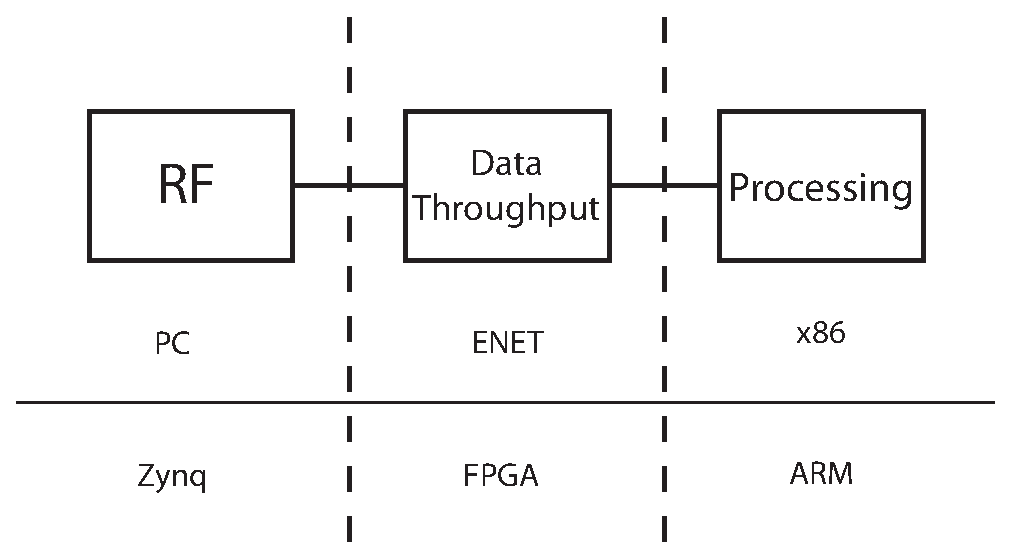
\includegraphics[width=4.0in]{Figures/architecture}}
\caption{}
\label{fig_arch}
\end{figure}

\subsection{Example Architecture under review}
\subsection{Important parameters}

\subsubsection{Pseudo Code}
\subsubsection{Signal Flow}
\subsubsection{Functionalities}

\section{Real World Challenges}
\subsection{Sampling speed}
\subsection{Non-linearities on the RF Frequency Response}
\subsection{SWAP}

\section{Results and Findings}

\section{Conclusions}

\bibliographystyle{IEEEtran}
\bibliography{IEEEabrv,commagbib}
\end{document}
